\documentclass{article}
\usepackage{graphicx}
\title{Graphical Representation of Heart Dataset}

\begin{document}
	\maketitle
	
	\begin{figure}[h]
		\centering
		\caption{\label{fig:gender_distribution}Heart Disease Distribution by Gender}
		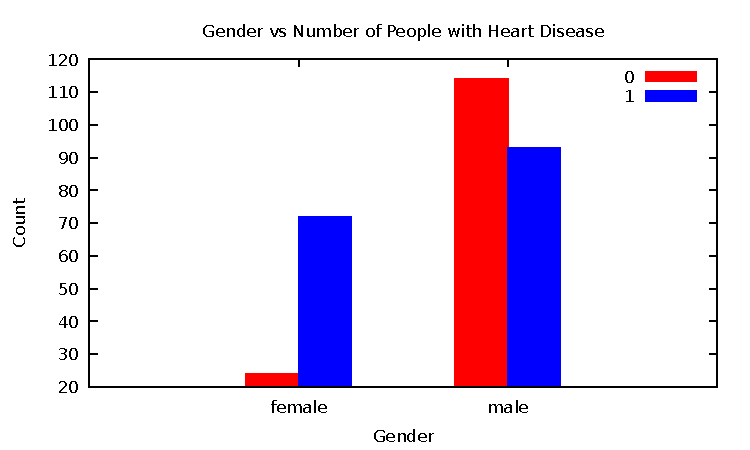
\includegraphics[scale=0.7]{que4a.pdf}
	\end{figure}
	
	\begin{figure}[h]
		\centering
		\caption{\label{fig:age_bp_correlation}Relationship between Age and Resting Blood Pressure}
		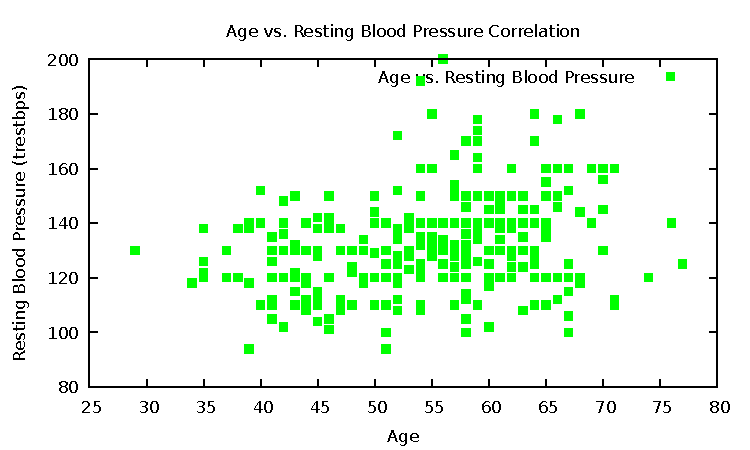
\includegraphics[scale=0.7]{age_bp_correlation.pdf}
	\end{figure}
	
	\begin{figure}[h]
		\centering
		\caption{\label{fig:age_cholesterol_no_disease}Age vs. Cholesterol Levels for Individuals without Heart Disease}
		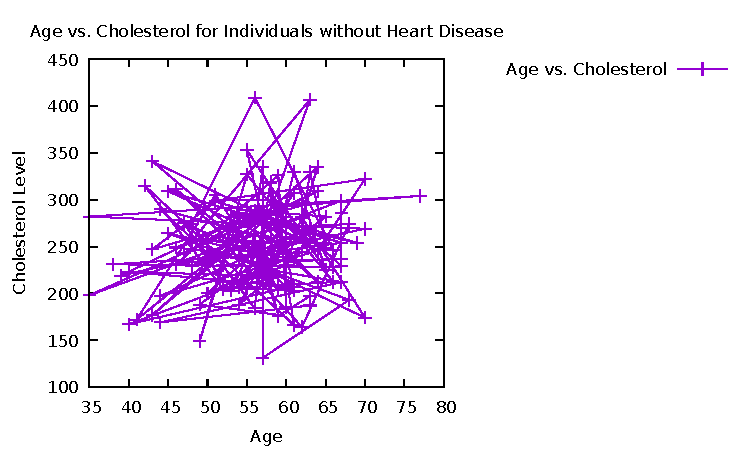
\includegraphics[scale=0.7]{age_cholesterol_chart.pdf}
	\end{figure}
	
	\begin{figure}[h]
		\centering
		\caption{\label{fig:age_group_distribution}Heart Disease Prevalence by Age Group (Pie Chart)}
		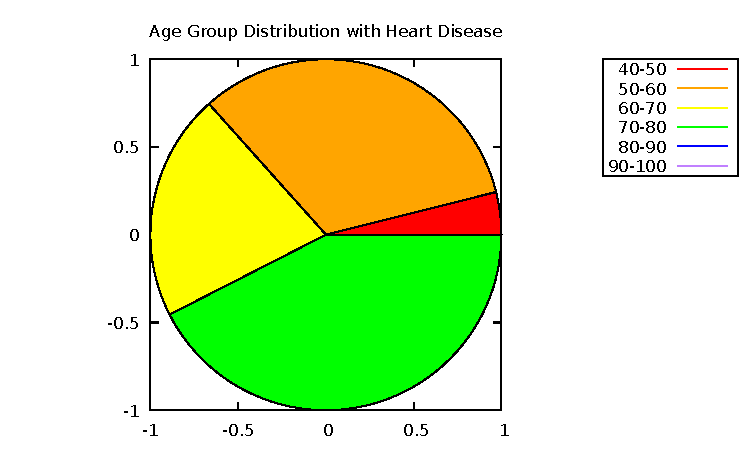
\includegraphics[scale=0.7]{age_groups_chart.pdf}
	\end{figure}
	
\end{document}
